\section{Hiện thực ứng dụng}
\label{results}

\subsection{Yêu cầu chung của bài toán}

Hệ thống được triển khai là một hệ thống đơn giản, chỉ bao gồm backend và database. Người dùng sử dụng một domain duy nhất truy cập vào ứng dụng. Tùy vị trí của người dùng, ứng dụng được điều hướng đến các server khác nhau. Ứng dụng có sử dụng cân bằng tải. Database có khả năng chịu lỗi cao, thời gian đọc nhanh.

\subsection{Phân tích thiết kế hệ thống}

\begin{figure}
    \centering
    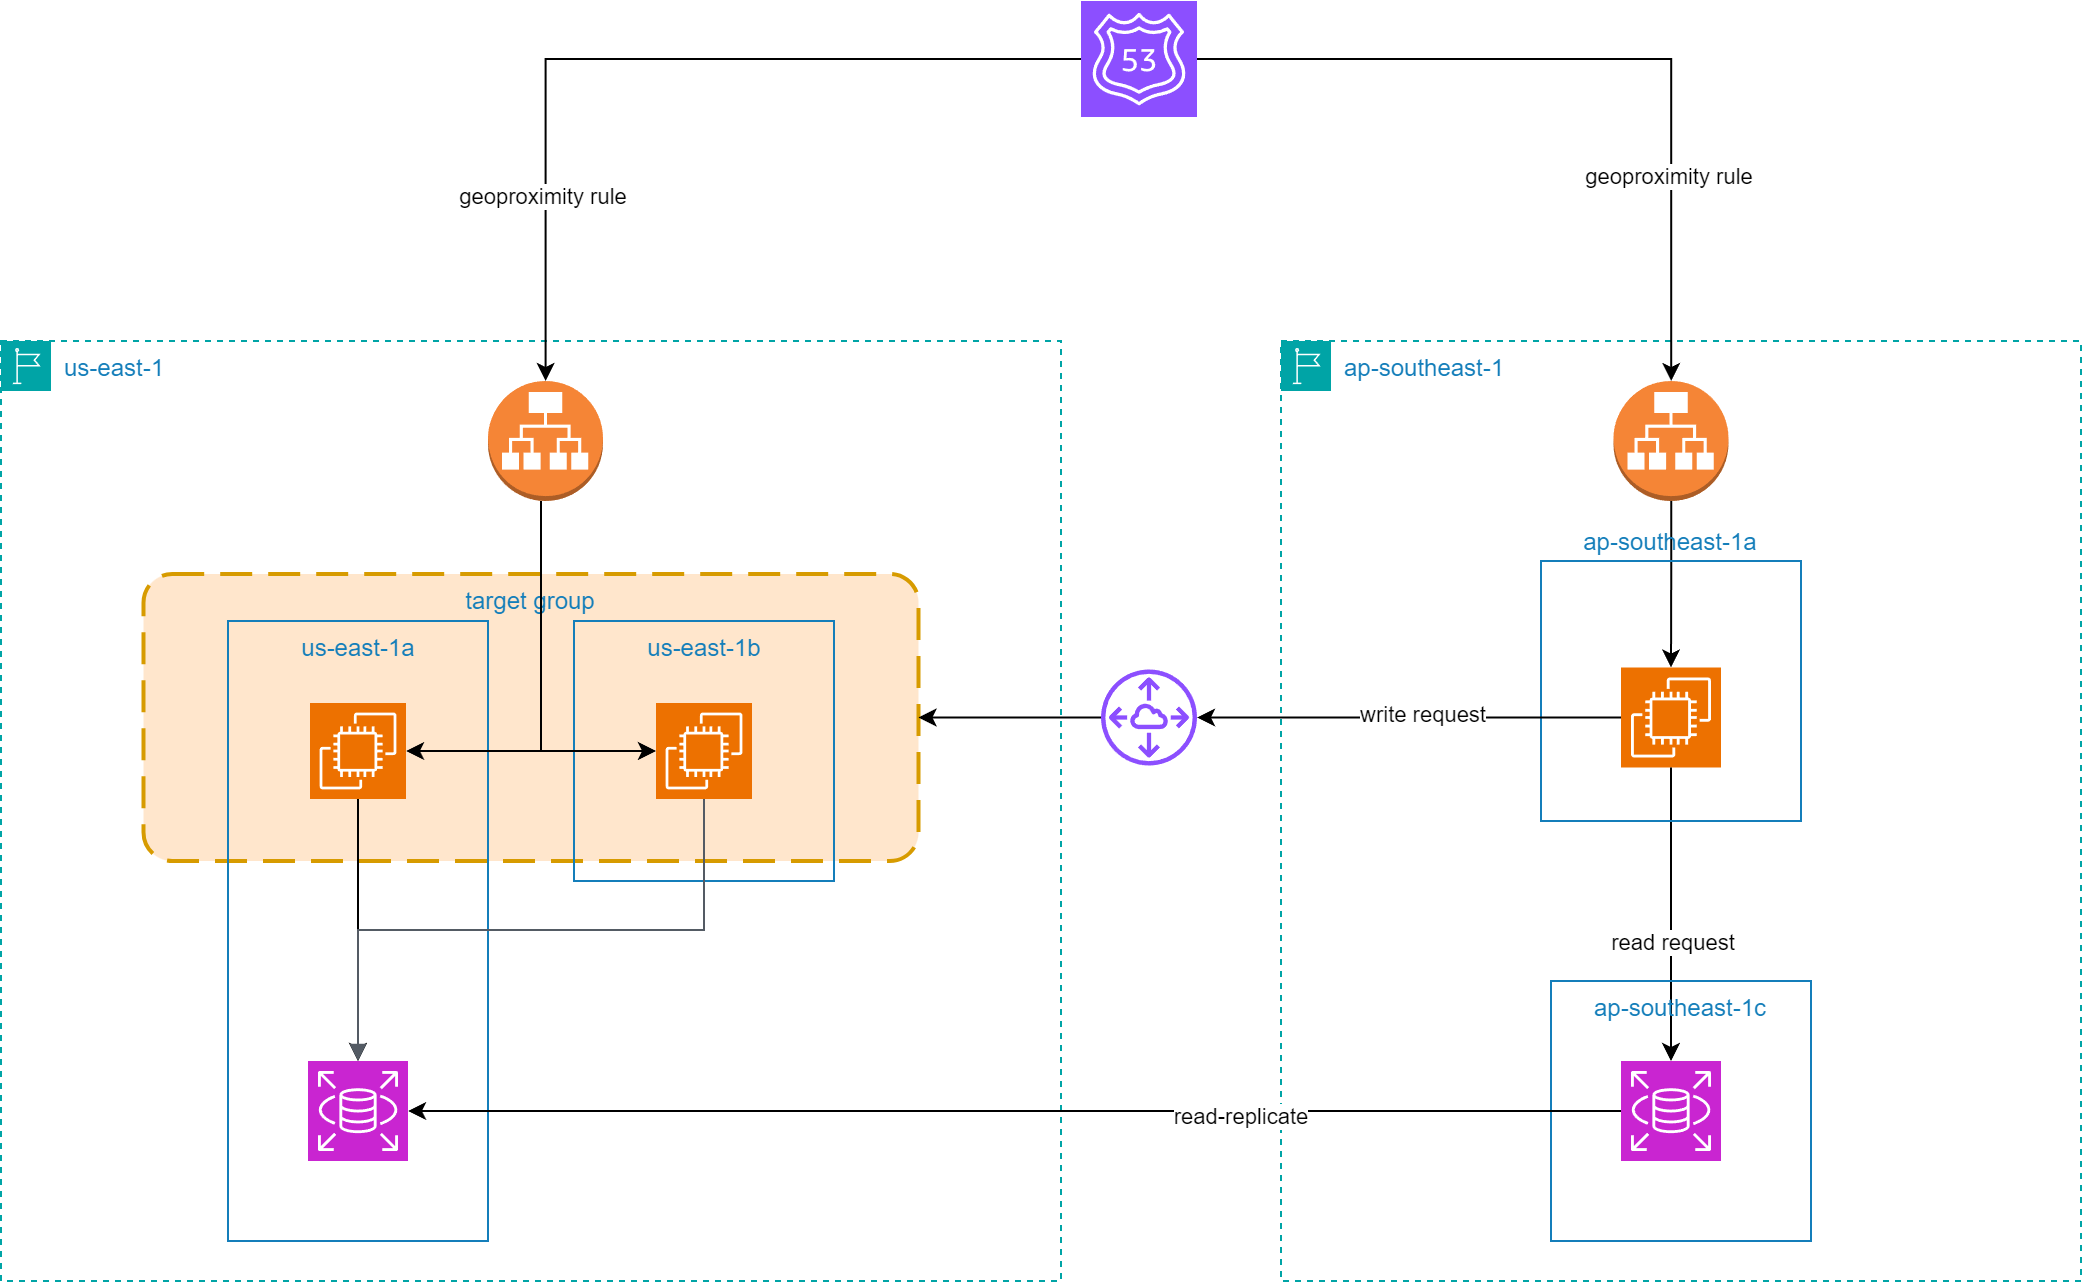
\includegraphics[scale=0.3]{../figures/section4/overall-diagram.png}
    \caption{Sơ đồ tổng quan ứng dụng}
    \label{fig:sec4-overall-diagram}
\end{figure}

\subsection{Hiện thực ứng dụng}

\subsection{Kết quả ứng dụng trong từng ngữ cảnh}